\chapter{Anwendungsfall und Prototyp}
\label{chapter:prototype}

In den Kapiteln zuvor wurde in das Thema durch Grundlagen und eine Vorstellung der einzelnen Streaming frameworks eingeführt. Das Kapitel \ref{chapter:prototype} beschreibt eine Methode zur Messung der Performance. Es wird zunächst das Messverfahren gezeigt und die Messumgebung beschrieben. Abschließend wird eine Messung durchgeführt und die Messergebnisse vorgestellt.

In der Abbildung \ref{fig:prototypeStreamingGraph} wird ein erster Bildschirmausschnitt aus einer Messung mit Apache Storm über ein Standardtestdatensatz für das Zählen von Worten gezeigt.

\begin{figure}[htb!]
\centering
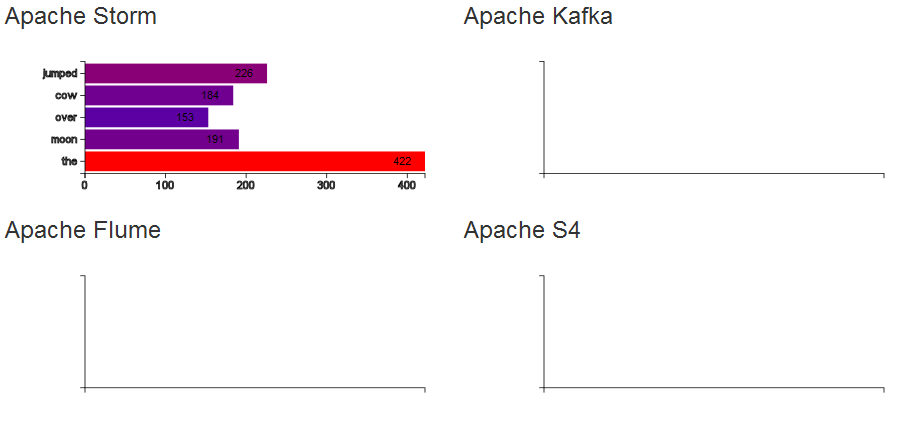
\includegraphics[width=1.0\textwidth]{bilder/PrototypeStreamingGraph.png}
\caption{Prototype Streaming Graph
\label{fig:prototypeStreamingGraph}}
\end{figure}


%STORM TRHOUGHPUT%
\begin{figure}
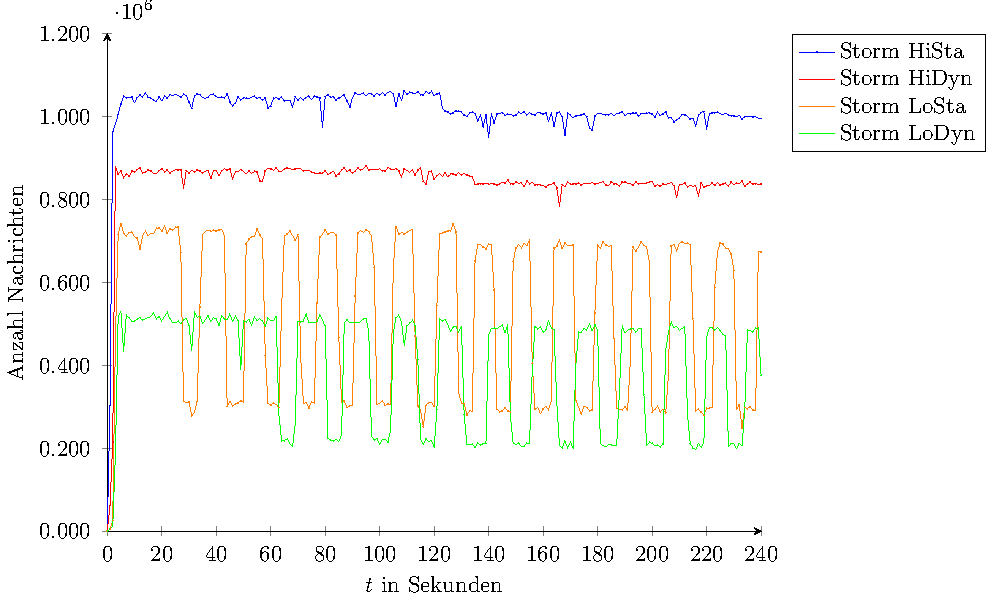
\includegraphics[width=0.97\textwidth]{plots/messungStormDurchsatz.pdf}
\caption{Messung Apache Storm Nachrichtendurchsatz
\label{fig:messungStormDurchsatz}}
\end{figure}
%STORM CPU%
\begin{figure}
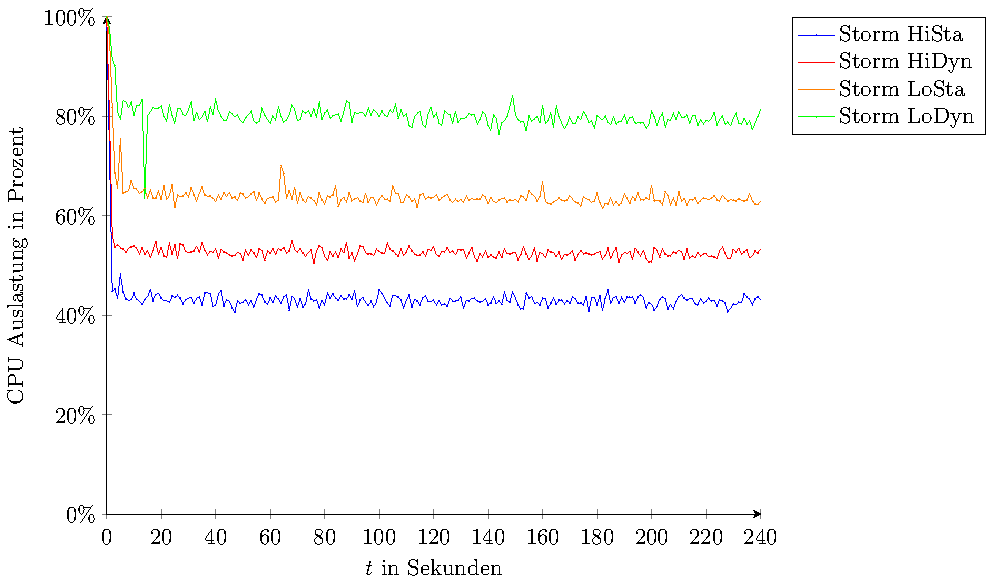
\includegraphics[width=0.97\textwidth]{plots/messungStormCpu.pdf}
\caption{Messung Apache Storm CPU Auslastung
\label{fig:messungStormCpu}}
\end{figure}


%KAFKA TRHOUGHPUT%
\begin{figure}
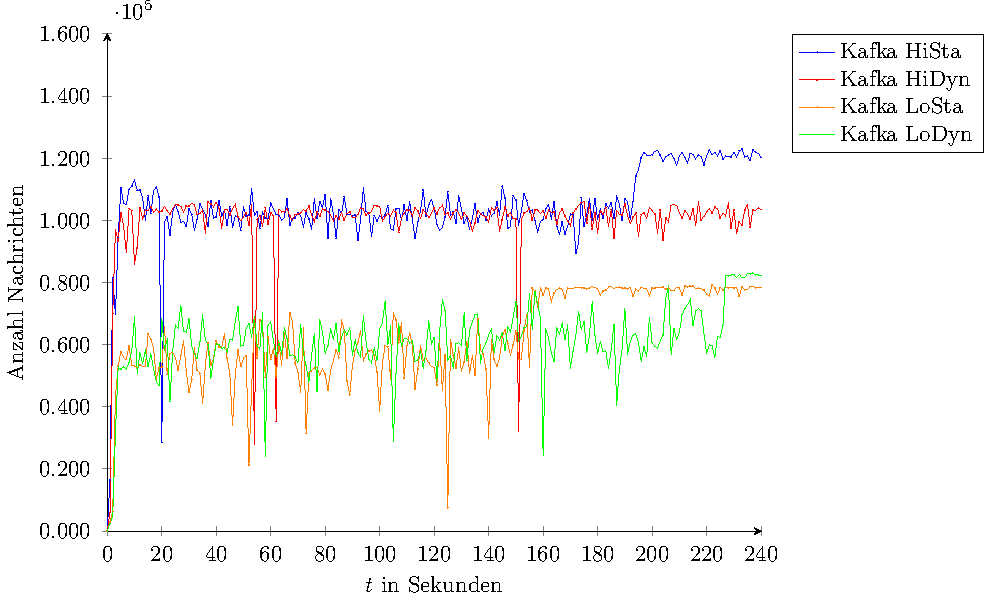
\includegraphics[width=0.97\textwidth]{plots/messungKafkaDurchsatz.pdf}
\caption{Messung Apache Kafka Nachrichtendurchsatz
\label{fig:messungKafkaNd}}
\end{figure}
%KAFKA CPU%
\begin{figure}
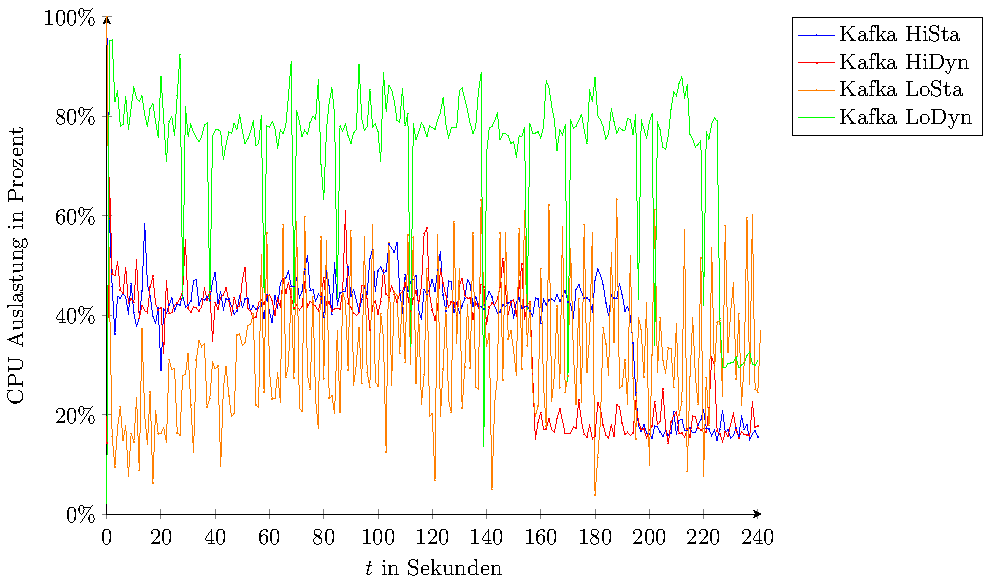
\includegraphics[width=0.97\textwidth]{plots/messungKafkaCpu.pdf}
\caption{Messung Apache Kafka CPU Auslastung
\label{fig:messungKafkaCpu}}
\end{figure}


%FLUME TRHOUGHPUT%
\begin{figure}
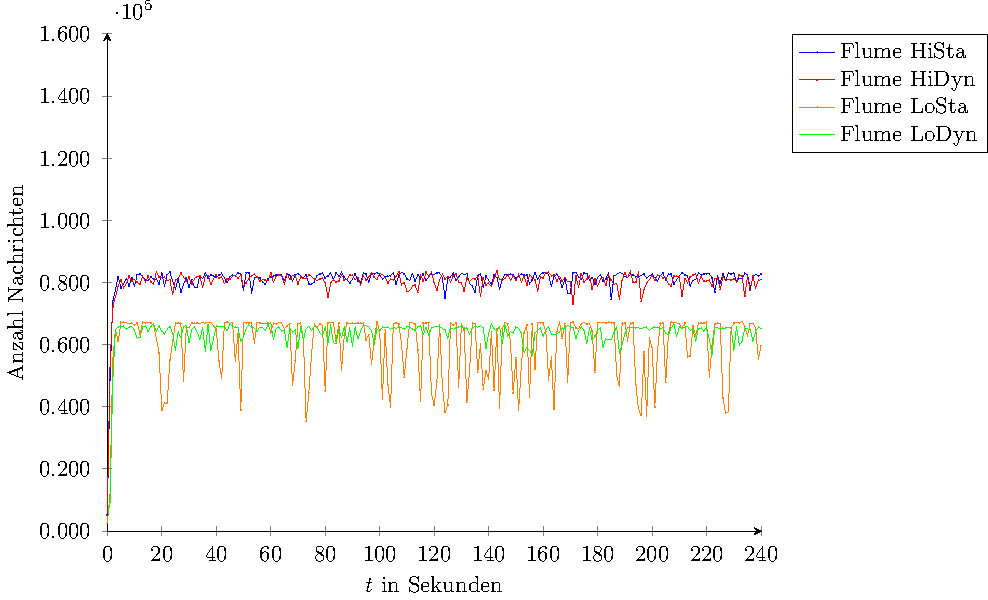
\includegraphics[width=0.97\textwidth]{plots/messungFlumeDurchsatz.pdf}
\caption{Messung Apache Flume Nachrichtendurchsatz
\label{fig:messungFlumeNd}}
\end{figure}
%FLUME CPU%
\begin{figure}
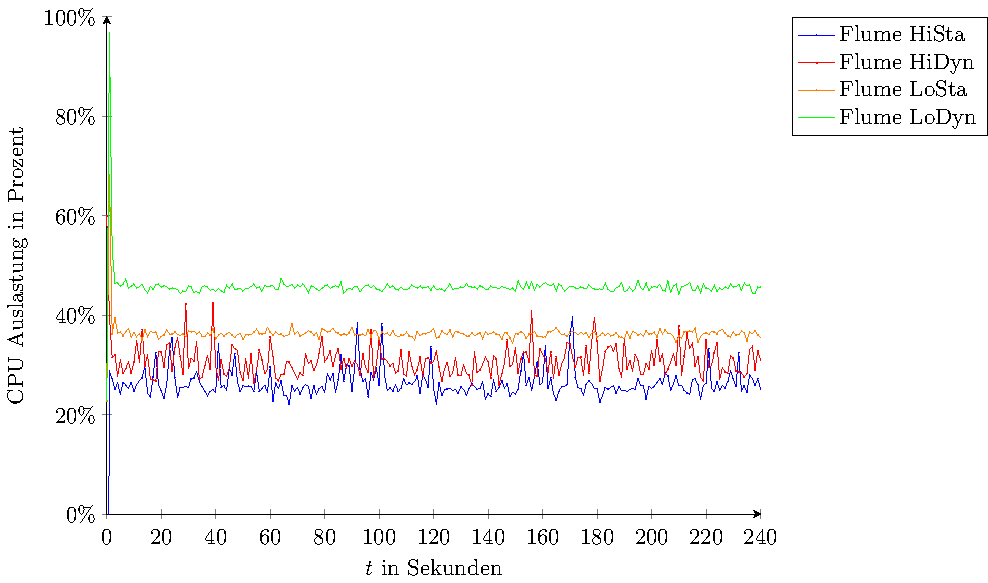
\includegraphics[width=0.97\textwidth]{plots/messungFlumeCpu.pdf}
\caption{Messung Apache Flume CPU Auslastung
\label{fig:messungFlumeCpu}}
\end{figure}


%Virtualbox RAW MEssung%
\begin{figure}
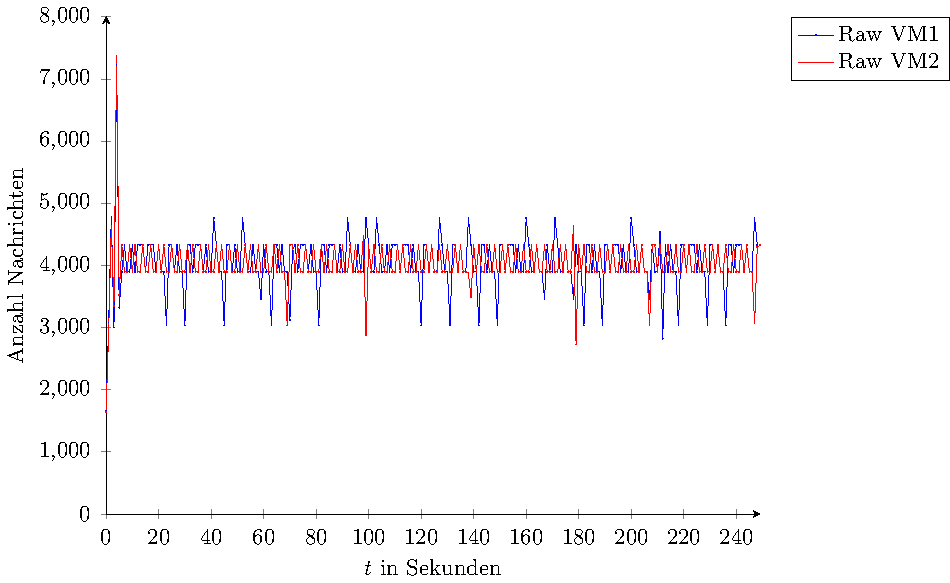
\includegraphics[width=1.0\textwidth]{plots/virtualBoxRaw.pdf}
\caption{Messung Nachrichtendurchsatz in Virtualbox
\label{fig:messungMaxNachrichten}}
\end{figure}

Dataset: \citeint{dataset:shakespeare:1994:CWW}